\chapter{مقدمه}
بر اساس قانون مور
\LTRfootnote{Moore's law}
قدرت پردازنده های کامپیوتر های کلاسیک هر دو سال، دو برابر میشود. اما این رویه تا حدی ادامه خواهد داشت که محدودیت های دنیای فیزیک کلاسیک به آن اجازه دهند. چرا که اندازه ی اعضای تشکیل دهنده ی پردازنده ها به حدی کوچک میشود که ناخودآگاه وارد فضای کوچک کوانتوم
\LTRfootnote{Quantum}
 میشوند. پیشبینی میشود این اتفاق در سال 2050 رخ دهد.
\\
 پیچیدگی محاسباتی
\LTRfootnote{Computational complexity}
 برخی الگوریتم ها در کامپیوتر های کلاسیک کمتر قابلیت کاهش ندارند. در حالی که کامپیوتر های کوانتومی، در تئوری میتوانند با مقدار بزرگی داده همانند یک واحد داده برخورد کنند و پیچیدگی محاسباتی الگوریتم ها را کاهش دهند.
\cite{singhbook1in2}
به طور کلی، محاسبات کوانتومی از کنش و واکنش مواد در جهان در سطح ذرات تشکیل دهنده ی آن بهره میگیرد و بر روی بستر پدیده ی نسبیت خاص
\LTRfootnote{Special relativity}
 پایه‌گذاری شده‌است. 
\\
برای مثال، کامپیوتر کلاسیک مشکلی در پیدا کردن نام فرد موردنظر در یک کتاب تلفن ندارند. اما برای مسائل ریاضی بهینه سازی پیچیده
\LTRfootnote{Complex mathematical optimizing}
  که مسائلی هستند که برای پیدا کردن حالت بهینه با توجه به متغیر های مختلف است، کامپیوتر های کلاسیک پاسخگو نیستند. از جمله این مسائل میتوان به اختصاص دادن منابع در ساخت یک برج بزرگ برای بدست آوردن کمترین خرج ممکن اشاره کرد.  چنین مسائلی در همه ی خوزه ها وجود دارند و کامپیوتر های کوانتومی برای اجرای این الگوریتم ها بسیار مناسب هستند. 
\cite{singhbook1in4}

‌\section{‌خواص دنیای محاسبات کوانتومی}
\subsection{کیوبیت}
کیوبیت ها
\LTRfootnote{Qubits}
 در کامپیوتر های کوانتومی، معادل بیت ها
\LTRfootnote{bits}
 در کامپیوتر های کلاسیک هستند. یک بیت یا در حالت صفر قرار دارد یا در حالت یک قرار دارد. تفاوت کیوبیت ها در این است که میتوانند حالی به جز صفر یا یک داشته باشند یا میتوان گفت برهم‌نهی 
\LTRfootnote{superposition}
حالات را شاهد هستیم. درنتیجه، کیوبیت میتواند حالات بیشتری از بیت داشته باشد. هر کیوبیت، به یک احتمالی میتواند یک باشد و به یک احتمالی میتواند صفر باشد. 
\begin{equation}
\left|\Psi\right\rangle = \alpha\left|0\right\rangle + \beta\left|1\right\rangle = \begin{bmatrix}
 \alpha
\\
\beta
\end{bmatrix}
\end{equation}
به طوری که 
$\alpha$
 و 
$\beta$
  شدت احتمال هستند و هر دو اعداد مختلط هستند به طوری که
\begin{equation}
\alpha^{2} + \beta^{2} = 1
\end{equation}
فضای حالتی که این دو متغیر تشکیل میدهند، یک فضای مختلط دو بعدی است.  حالات خاص صفر و یک، یک فضای بردار پایه ای
\LTRfootnote{orthonormal basis}
برای این فضای برداری تشکیل میدهند.
\begin{equation}
\left|0\right\rangle = (0, 1) and \left|1\right\rangle = (1, 0)
\end{equation}
در شکل پایین، میتوانید کره ی بلاچ
\LTRfootnote{Bloch's sphere}
  که نوعی بازنمایی هندسی از حالت یک کیوبیت است، را مشاهده کنید.
\begin{figure}[!h]
\centerline{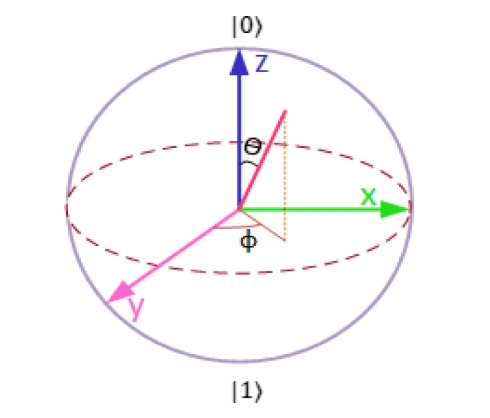
\includegraphics[width=.5\textwidth]{bloch.jpeg}}
\caption{بازنمایی کیوبیت در کره بلاچ}
\end{figure}
این بازنمایی را میتوانید به تعداد نامحدودی کیوبیت هم انطباق دهید. به طوری که با داشتن $n$ کیوبیت نیاز به نگهداری $n^{2}$ عدد خواهید داشت. این حالت زمانی رخ میدهد که $n$ کیوبیت درهم‌تنیده
\LTRfootnote{entangled}
 شوند به طوری که باهم یک حالت را تشکیل دهند و نتوان آن ها را جدا کرد. 
\cite{fundamentalsandapplications}
همچنان جمع مجذور همه ی مقادیر باید برابر با یک شود. نمایش انتزاعی دو کیوبیت به شکل زیر خواهد بود:
\begin{equation}
\left|\Psi\right\rangle = \alpha_{0}\left|00\right\rangle +  \alpha_{1}\left|01\right\rangle +  \alpha_{2}\left|10\right\rangle +  \alpha_{3}\left|11\right\rangle = \begin{bmatrix}
 \alpha_{0}
\\
 \alpha_{1}
\\
 \alpha_{2}
\\
 \alpha_{3}
\end{bmatrix}
\end{equation}
نمایش دو کیوبیت در فرم ماتریسی و دیراک
\LTRfootnote{Dirac}
:
\begin{equation}
\left|00\right\rangle  = \begin{bmatrix}
 \alpha_{1}
\\
 \alpha_{0}
\\
 \alpha_{0}
\\
 \alpha_{0}
\end{bmatrix}
\text{;}
\left|01\right\rangle  = \begin{bmatrix}
 \alpha_{0}
\\
 \alpha_{1}
\\
 \alpha_{0}
\\
 \alpha_{0}
\end{bmatrix}
\text{;}
\left|10\right\rangle  = \begin{bmatrix}
 \alpha_{0}
\\
 \alpha_{0}
\\
 \alpha_{1}
\\
 \alpha_{0}
\end{bmatrix}
\text{;}
\left|11\right\rangle  = \begin{bmatrix}
 \alpha_{0}
\\
 \alpha_{0}
\\
 \alpha_{0}
\\
 \alpha_{1}
\end{bmatrix}
\end{equation}


\subsection{ضرب تانسوری}
ضرب تانسوری
\LTRfootnote{Tensor product}
، عملیاتی است که بین دو ماتریس میتوان انجام داد. این عملیات، یکی از بخش های اصلی محاسبات کوانتومی است. برای اینکه بتوان سیستم های چند-کیوبیتی
\LTRfootnote{multiple-qubit systems}
را به صورت ریاضی نمایش داد، از این عملیات استفاده میشود. به این صورت که اگر $M$ یک ماتریس $(p,q)$ باشد و  $N$ یک ماتریس $(x,y)$ باشد، ماتریس ضرب تانسوری آنها یک ماتریس $(px,qy)$ خواهد بود. 
\cite{fundamentalsandapplications}
این ضرب را میتوان با یک گیت کوانتومی
\LTRfootnote{quantum gate}
 اعمال کرد.
\begin{equation}
M =  \begin{bmatrix}
 a_{11} &  a_{12}
\\
 a_{21} & a_{22}
\end{bmatrix}
\text{;}
N =  \begin{bmatrix}
 b_{11} &  b_{12}
\\
 b_{21} &  b_{22}
\end{bmatrix}
\end{equation}

\begin{equation}
M \oplus  N =  \begin{bmatrix}
 a_{11}b_{11} &  a_{11}b_{12} &  a_{12}b_{11} &  a_{12}b_{12}
\\
 a_{11}b_{21} &  a_{11}b_{22} &  a_{12}b_{21} &  a_{12}b_{22}
\\
 a_{21}b_{11} &  a_{21}b_{12} &  a_{22}b_{11} &  a_{22}b_{12}
\\
 a_{21}b_{21} &  a_{21}b_{22} &  a_{22}b_{21} &  a_{22}b_{22}
\end{bmatrix}
\end{equation}
برای ضرب تانسوری دو کیوبیت خواهیم داشت:
\begin{equation}
\left|0\right\rangle  \oplus  \left|1\right\rangle  =
\begin{bmatrix}
1 \\ 0 
\end{bmatrix} 
\oplus 
\begin{bmatrix}
0 \\ 1 
\end{bmatrix} 
=
  \begin{bmatrix}
0
\\
1
\\
0
\\
0
\end{bmatrix} = \left|01\right\rangle
\end{equation}
